\documentclass{article}
\usepackage{tikz}
\usepackage{amsmath}
\usetikzlibrary{calc} % Libreria per il calcolo delle coordinate
\usetikzlibrary{scopes}
\begin{document}
\section{peso su piano e forza}
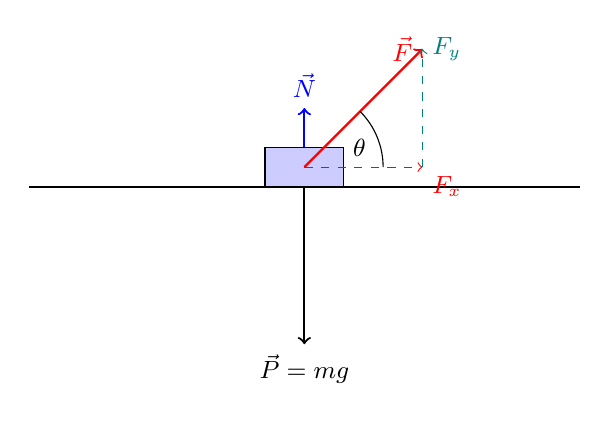
\begin{tikzpicture}[font = \small]
  % Disegna il piano orizzontale
  \draw[thick] (-1,0) -- (6,0);

  % Posizione del corpo
  \coordinate (A) at (2,0);

  % Disegna il corpo (un rettangolo)
  \draw[fill=blue!20] (A) rectangle ++(1,0.5);

  % Peso (forza gravitazionale)
  \draw[->, thick] ($(A)+(0.5,0)$) -- ++(0,-2) node[below] {$\vec{P} = mg$};

  % Forza applicata
  \draw[->, thick, red] ($(A)+(0.5,0.25)$) -- ++(1.5,1.5) node[ left] {$\vec{F}$};

  % Scomposizione della forza applicata
  % \draw[dashed, red] ($(A)+(0.5,0.25)$) -- ++(1.5,0);
  % \draw[dashed, red] ($(A)+(2.5,0.25)$) -- ++(0,1.5);

  % Componenti della forza applicata
  \draw[->, dashed, red] ($(A)+(0.5,0.25)$) -- ++(1.5,0) node[below right] {$F_x$};
  \draw[->, dashed, teal] ($(A)+(2,0.25)$) -- ++(0,1.5) node[right] {$F_y$};

  % Reazione vincolare
  \draw[->, thick, blue] ($(A)+(0.5,0.5)$) -- ++(0,0.5) node[above] {$\vec{N}$};

  % Angolo theta
  \draw ($(A)+(1.5,0.25)$) arc (0:45:1);
  \node at ($(A)+(1.2,0.5)$) {$\theta$};
\end{tikzpicture}

\section{oggetto appeso a due cavi}
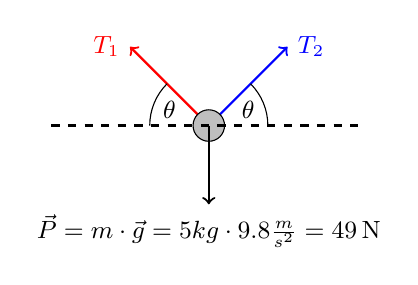
\begin{tikzpicture}[font = \small]
  % Posizione del punto di sospensione e massa
  % \coordinate (O) at (0,0); % Punto di sospensione
  \coordinate (A) at (-1,-2); % Punto in cui termina il cavo sinistro
  \coordinate (B) at (1,-2); % Punto in cui termina il cavo destro
  \coordinate (M) at (0,-3); % Massa

  % Disegna i cavi (dalla massa verso l'alto)
  \draw[->, thick, red] (M) -- (A) node[  left] {$T_1$};
  \draw[->, thick, blue] (M) -- (B) node[  right] {$T_2$};

  % Disegna la massa
  \draw[fill=gray!50] (M) circle (0.2) ;

  %disegna il piano orizzonatle
  \draw[dashed, thick] (-2,-3) -- (2,-3);

  % Disegna la forza peso
  \draw[->, thick, black] (M) -- ++(0,-1) node[below] {$\vec{P} = m\cdot \vec{g} = 5 kg \cdot 9.8 \frac{m}{s^2} = 49\,\text{N}$};

  % Componenti delle tensioni
  % \draw[dashed, red] (M) -- ($(M)!0.7!(A)$ |- M) node[midway, left] {$T_1 \sin\theta$};
  % \draw[dashed, blue] (M) -- ($(M)!0.7!(B)$ |- M) node[midway, right] {$T_2 \sin\theta$};

  % \draw[dashed, red] ($(M)!0.7!(A)$ |- M) -- ($(M)!0.7!(A)$) node[midway, above] {$T_1 \cos\theta$};
  % \draw[dashed, blue] ($(M)!0.7!(B)$ |- M) -- ($(M)!0.7!(B)$) node[midway, above] {$T_2 \cos\theta$};

  % Punto di sospensione
  % \fill[black] (O) circle (0.1);

  % Angoli theta
  \draw (M) ++ (-0.75,0) arc[start angle=180, end angle=135, radius=0.75];
  \node at (-0.5,-2.8) {$\theta$};

  \draw (M) ++(0.75,0) arc[start angle=0, end angle=45, radius=0.75];
  \node at (0.5,-2.8) {$\theta$};
\end{tikzpicture}

\section{corpo appeso}
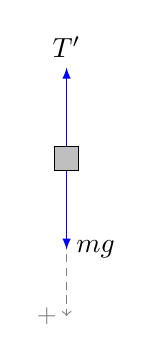
\begin{tikzpicture}[
    force/.style={>=latex,draw=blue,fill=blue},
    axis/.style={densely dashed,gray,font=\small},
    M/.style={rectangle,draw,fill=lightgray,minimum size=0.5cm,thin},
    m/.style={rectangle,draw=black,fill=lightgray,minimum size=0.3cm,thin},
    plane/.style={draw=black,fill=blue!10},
    string/.style={draw=red, thick},
    pulley/.style={thick},
]
    % Free body diagram of m
    \node[m] (m) {};
    \draw[axis,->] (m) -- ++(0,-2) node[left] {$+$};
    {[force,->]
        \draw (m.north) -- ++(0,1) node[above] {$T'$};
        \draw (m.south) -- ++(0,-1) node[right] {$mg$};
    }
\end{tikzpicture}



\end{document}